\chapter{Architektur}
\section{Modularisierung}
An vielen Stellen der Privacy-Crash-Cam bietet sich eine Modularisierung an. D.h. in sich geschlossene Programmabschnitte werden voneinander getrennt und kommunizieren über vereinbarte Schnittstellen~\eqref{allg:Rest}. Dies bietet eine Reihe von Vorteilen:
\begin{itemize}
\itemsep0pt
\item Reduziert die Koordination und Kommunikation und verringert dadurch die Komplexität.
\item Höhere Flexibilität, da nur einzelne Module an neue Bedingungen (z.B. andere Plattformen) angepasst werden müssen.
\item Höhere Wiederverwertbarkeit, da einzelne Module in neue Systeme eingebunden werden können.
\item Bessere Austauschbarkeit, da einfach einzelne Module ausgetauscht werden können, solange sie die Schnittstellen beachten.
\item Schnellere Fehlersuche, da der Suchbereich eingeschränkt werden kann.
\end{itemize}

In der Privacy-Crash-Cam findet eine Modularisierung durch vier Maßnahmen statt. 1. \nameref{allg:Komponenten}, 2. \nameref{allg:MVP}, 3. Modularisierung innerhalb der Komponenten (\eqref{app:modul},~\eqref{service:modul},~\eqref{interface:modul}) und 4. \nameref{allg:Entwurfsmuster}

\section{Trennung in Komponenten} \label{allg:Komponenten}

Die Privacy-Crash-Cam ist in drei Komponenten aufgeteilt. Die \nameref{chap:app}, den \nameref{chap:service} und das \nameref{chap:interface}. \newline
Da die App und die Webanwendung auf unterschiedlichen Technologien basieren, ist es natürlich diese Komponenten getrennt zu entwickeln. Zudem entsteht eine erhöhte Flexibilität, da so z.B. erlaubt wird die App auch für andere Betriebssysteme zu entwickeln als Android, ohne die Webanwendung zu verändern. \newline
Zusätzlich wird die Webanwendung in Web-Dienst und Web-Interface unterteilt, um die logisch voneinander unabhängigen Komponenten App und Web-Interface zu trennen.

\section{Model View Presenter (MVP)} \label{allg:MVP}

Beim Design der Privacy-Crash-Cam wird schnell deutlich, dass eine strikte Trennung zwischen Datenbank, Applikationslogik und Benutzeroberfläche von Vorteil ist. Das Model-View-Presenter-Prinzip (kurz: MVP) realisiert diese Trennung und wird auf auf App und Webanwendung eingesetzt.\newline\par

\begin{figure}[ht]
	\centering
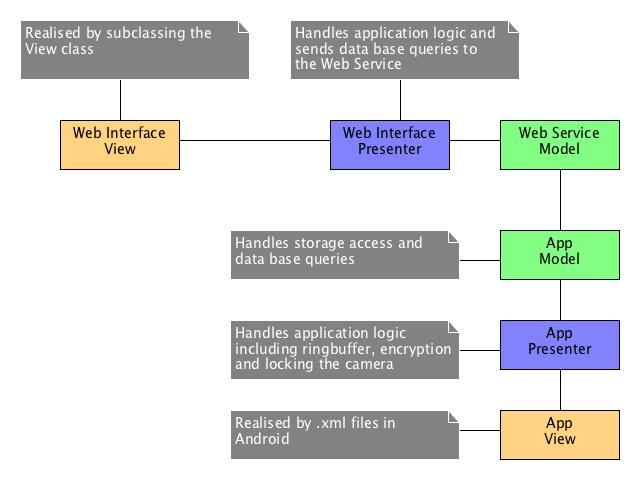
\includegraphics[width=1\textwidth]{./resources/Diagramme/overview_mvp.jpg}
\caption{MVP in der Privacy Crash Cam}
	\label{fig:overview_mvp}
\end{figure}

Sowohl App, als auch Web-Interface besitzen ein eigenes View-Modul. Dieses ist für die graphische Benutzeroberfläche zuständig. In der App wird die View durch XML-Dokumente und Activities implementiert, die das Layout definieren. Das Web-Interface verwendet dafür die von Vaadin bereitgestellte View-Klasse, von der man eigene Klassen ableiten kann.\newline\par

Die Applikationslogik wird durch die Presenter-Ebene umgesetzt. App und Web-Interface besitzen eigene Presenter-Module, die an die jeweilige Plattform angepasst sind. Der Presenter handhabt Eingaben durch Nutzer oder Sensoren und koordiniert die darauf folgenden Aktionen, wie das Aktualisieren der Ansichten und Änderungen des Models.\newline\par

Das Model ist dafür zuständig, Daten zu verwalten und zu bearbeiten. Die App hat dafür ein eigenes Modul, das den Speicherzugriff regelt. Das Model des Web-Interfaces ist der Web-Dienst, der alle Videodaten verwaltet.\newline\par

\section{TODO: Rest-API} \label{allg:Rest}
TODO!!

\section{Entwurfsmuster} \label{allg:Entwurfsmuster}
Der Einsatz weiterer Enwurfsmuster innerhalb der Module erleichtert die Lesbarkeit und begünstigt die Flexibilität des Codes noch weiter. Eingesetzte Muster sind in den entsprechenden Kapiteln für App~\eqref{chap:app}, Web Interface~\eqref{chap:interface} und Web Dienst~\eqref{chap:service} genauer beschrieben.